\chapter{User study} \label{chapter3}

Before designing the application, we needed to find out more about the needs and wants of students enrolled at \acrshort{acs} and the general context in which this application would function.

\section{Methods} \label{3:methods}

The research and data collection methods we used were \textbf{observation} (throughout the four years that the main author of the paper was enrolled at our faculty of choice, \acrshort{acs}), \textbf{interviews} (with students, professors as well as administrative personnel of the faculty) and a \textbf{survey}, the results of which we will be focusing on in this chapter.  We mention and discuss the results of the first two methods throughout the whole paper, where they offer insightful information for the specific section. Additionally, throughout every step of the whole process of designing the application, we went through a \textbf{feedback loop} with a small group of students to ensure that we were progressing in the right direction.

Partly due to the pandemic, the main method of communication with our potential users was online communication. Most of the interviews were done either via video call (through \textit{Microsoft Teams}\footnote{https://teams.microsoft.com/}) or via chat (\textit{Facebook Messenger}\footnote{https://messenger.com/}, \textit{WhatsApp}\footnote{https://www.whatsapp.com/}) or e-mail (\textit{Gmail}\footnote{http://gmail.com/}). The survey was a \textit{Google Form}\footnote{http://forms.google.com/} shared both verbally and through social media platforms, receiving 212 responses between October and December 2019. Since we regrettably could not gather a relevant number of responses from Master's students, with only seven responses, we will be focusing on the Bachelor's students, since 200 out of the total of about 600 enrolled B.Sc. students is statistically relevant.

To analyze the data, we imported the results from the form into a database using \textit{Microsoft SQL Server}\footnote{https://www.microsoft.com/en-us/sql-server/}, normalized the data and created visualizations using \textit{Microsoft Power BI}\footnote{https://powerbi.microsoft.com/}.

\section{Target audience} \label{3:target_audience}

Studies\cite{hammer2011importance}\cite{connelly2013demographic} show that demographic information in surveys helps to avoid bias towards a specific section of the target audience. Therefore, we included some \textbf{demographic questions} to ensure that the pool of respondents is relatively balanced.

In terms of \textbf{gender demographics}, our results (fig. \ref{3:fig:gender}) closely match a separate study\cite{codette2019stats} that is specifically targeting gender demographics at computer science faculties in Romania, including \acrshort{acs}.

\begin{figure}[ht]
    \centering
         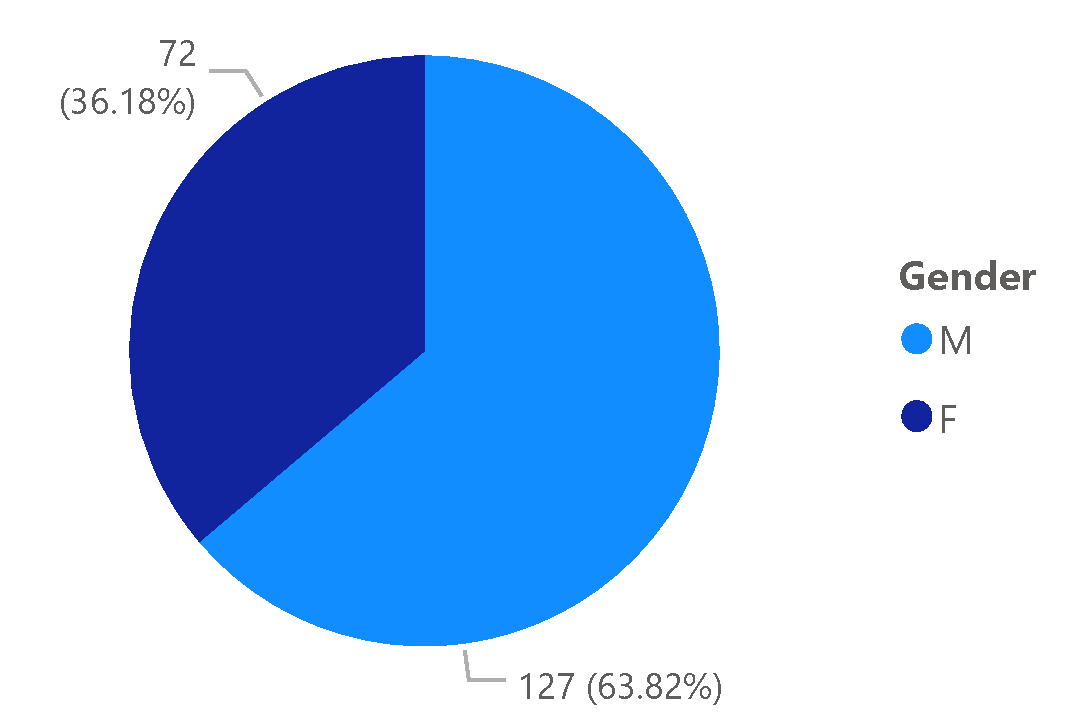
\includegraphics[height=0.2\textheight]{figures/charts/survey/gender.pdf}
    \caption{Gender of survey respondents}
    \label{3:fig:gender}
\end{figure}

Concerning \textbf{academic distribution}, we have received four times more responses from students pursuing the Computer Science domain (Computers and Information Technology, or CTI) than the Automatics domain (Systems Engineering, or IS), as seen in figure \ref{3:fig:domain}. Some discrepancy is expected, considering there are twice as many enrolled CTI students than IS students, according to the same study\cite{codette2019stats} mentioned above. The distribution of the respondents' year of study is relatively balanced (fig. \ref{3:fig:year}).

\begin{figure}[!ht]
    \centering
    \begin{minipage}[b]{0.49\textwidth}
        \captionsetup{justification=centering}
         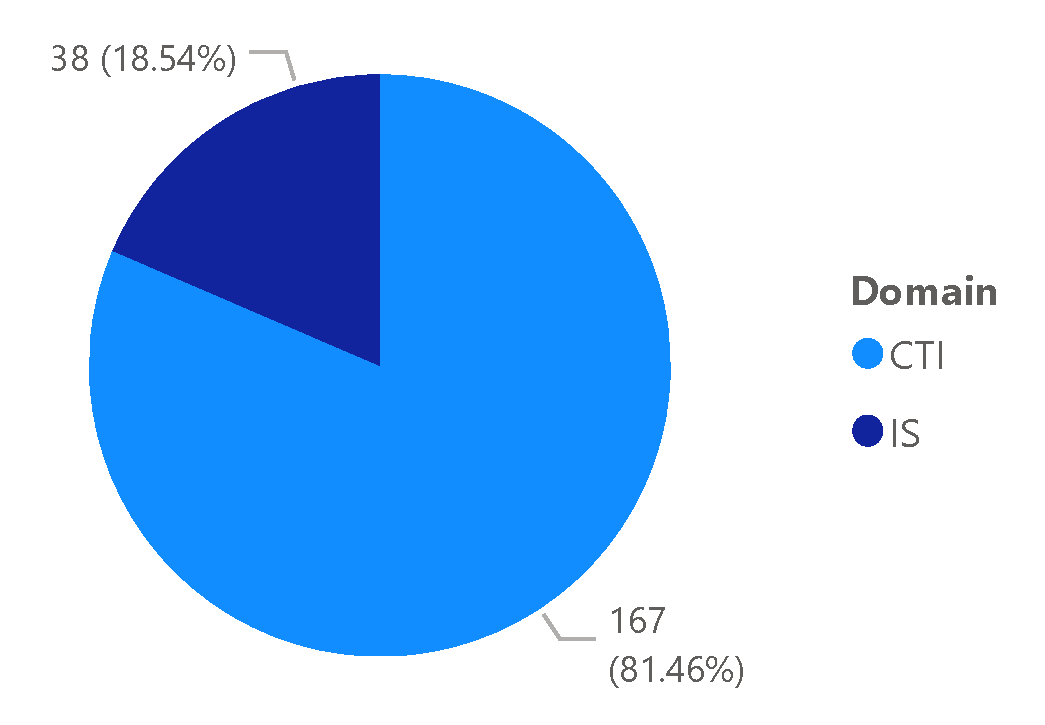
\includegraphics[height=0.2\textheight]{figures/charts/survey/domain.pdf}
        \caption{Domain of survey respondents}
        \label{3:fig:domain}
    \end{minipage}
    \hfill
    \begin{minipage}[b]{0.49\textwidth}
        \captionsetup{justification=centering}
         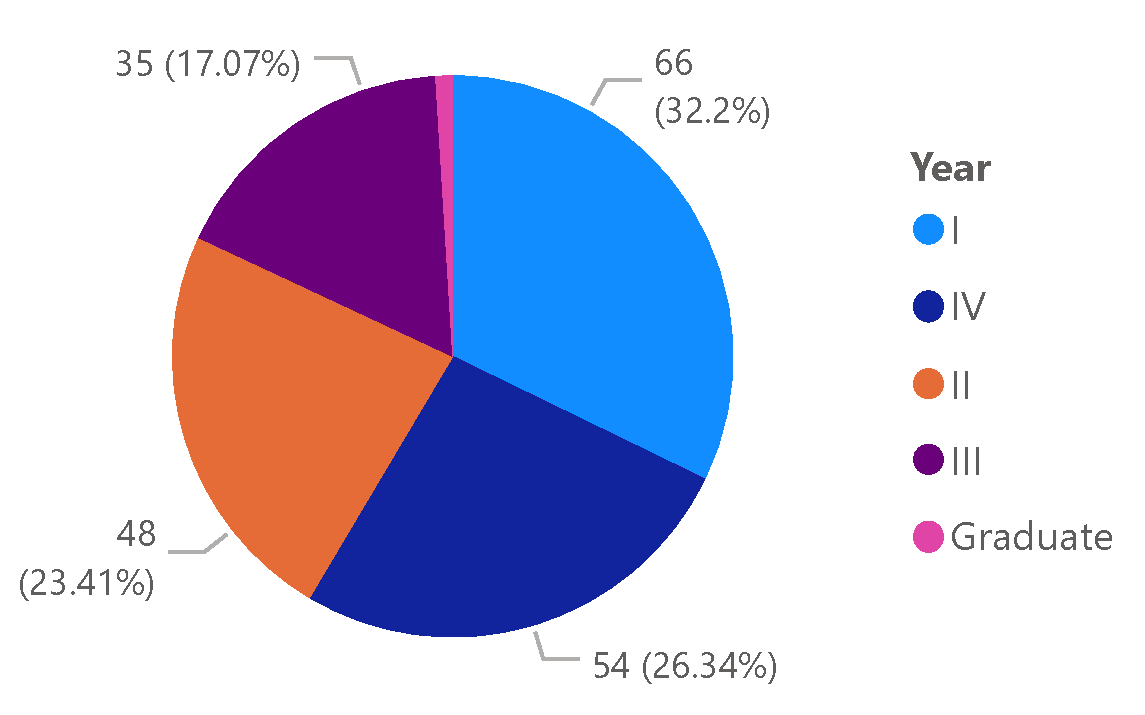
\includegraphics[height=0.2\textheight]{figures/charts/survey/year.pdf}
        \caption{Academic year of survey respondents}
        \label{3:fig:year}
    \end{minipage}
\end{figure}

Regarding \textbf{mobile operating systems}, the distribution is very similar to the Romanian mobile operating system market share, according to StatCounter GlobalStats \cite{statcounter2020mobile}, with 80\% of students using Android and 20\% of students using iOS.

\begin{figure}[ht]
    \centering
         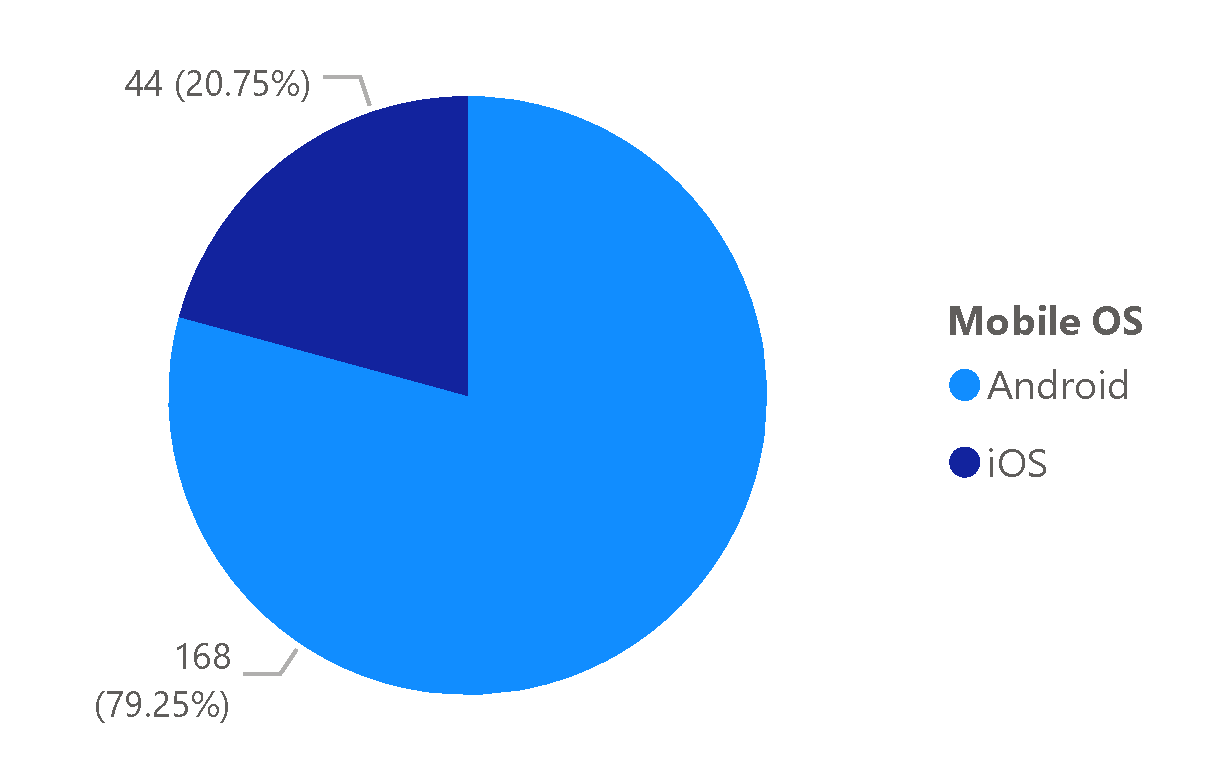
\includegraphics[height=0.2\textheight]{figures/charts/survey/os.pdf}
    \caption{Mobile \acrshort{os} of survey respondents}
    \label{3:fig:os}
\end{figure}

Upon reviewing the data, we believe that, aside from the lack of representation for Master's students, the respondents' demographics are varied enough for a relevant sample group. Since the student group we expect the app to be the most useful for is first-year B.Sc. students, we will be focusing more on their needs, since the app can be further extended in the future to meet the needs of older students, where these needs differ.

\section{Results} \label{3:results}

We used a variety of questions to learn more about the student's preferences and what they would be looking for in a university mobile application. For this purpose, we included \textbf{multiple-choice questions}, \textbf{Likert scale questions} and \textbf{open-ended questions} in the survey.

\subsection{Features} \label{3:features}

The survey's primary purpose was to find out what kind of features would be the most useful for our students. We provided a list of potential features or types of information that could be available in the application. We asked them to give each of them a rating from 1 (not very useful) to 5 (very useful). We devised a scoring system, with points between -2 and +3 for each answer, and came up with the hierarchy seen in figure \ref{3:fig:features}.

\begin{figure}[ht]
    \centering
         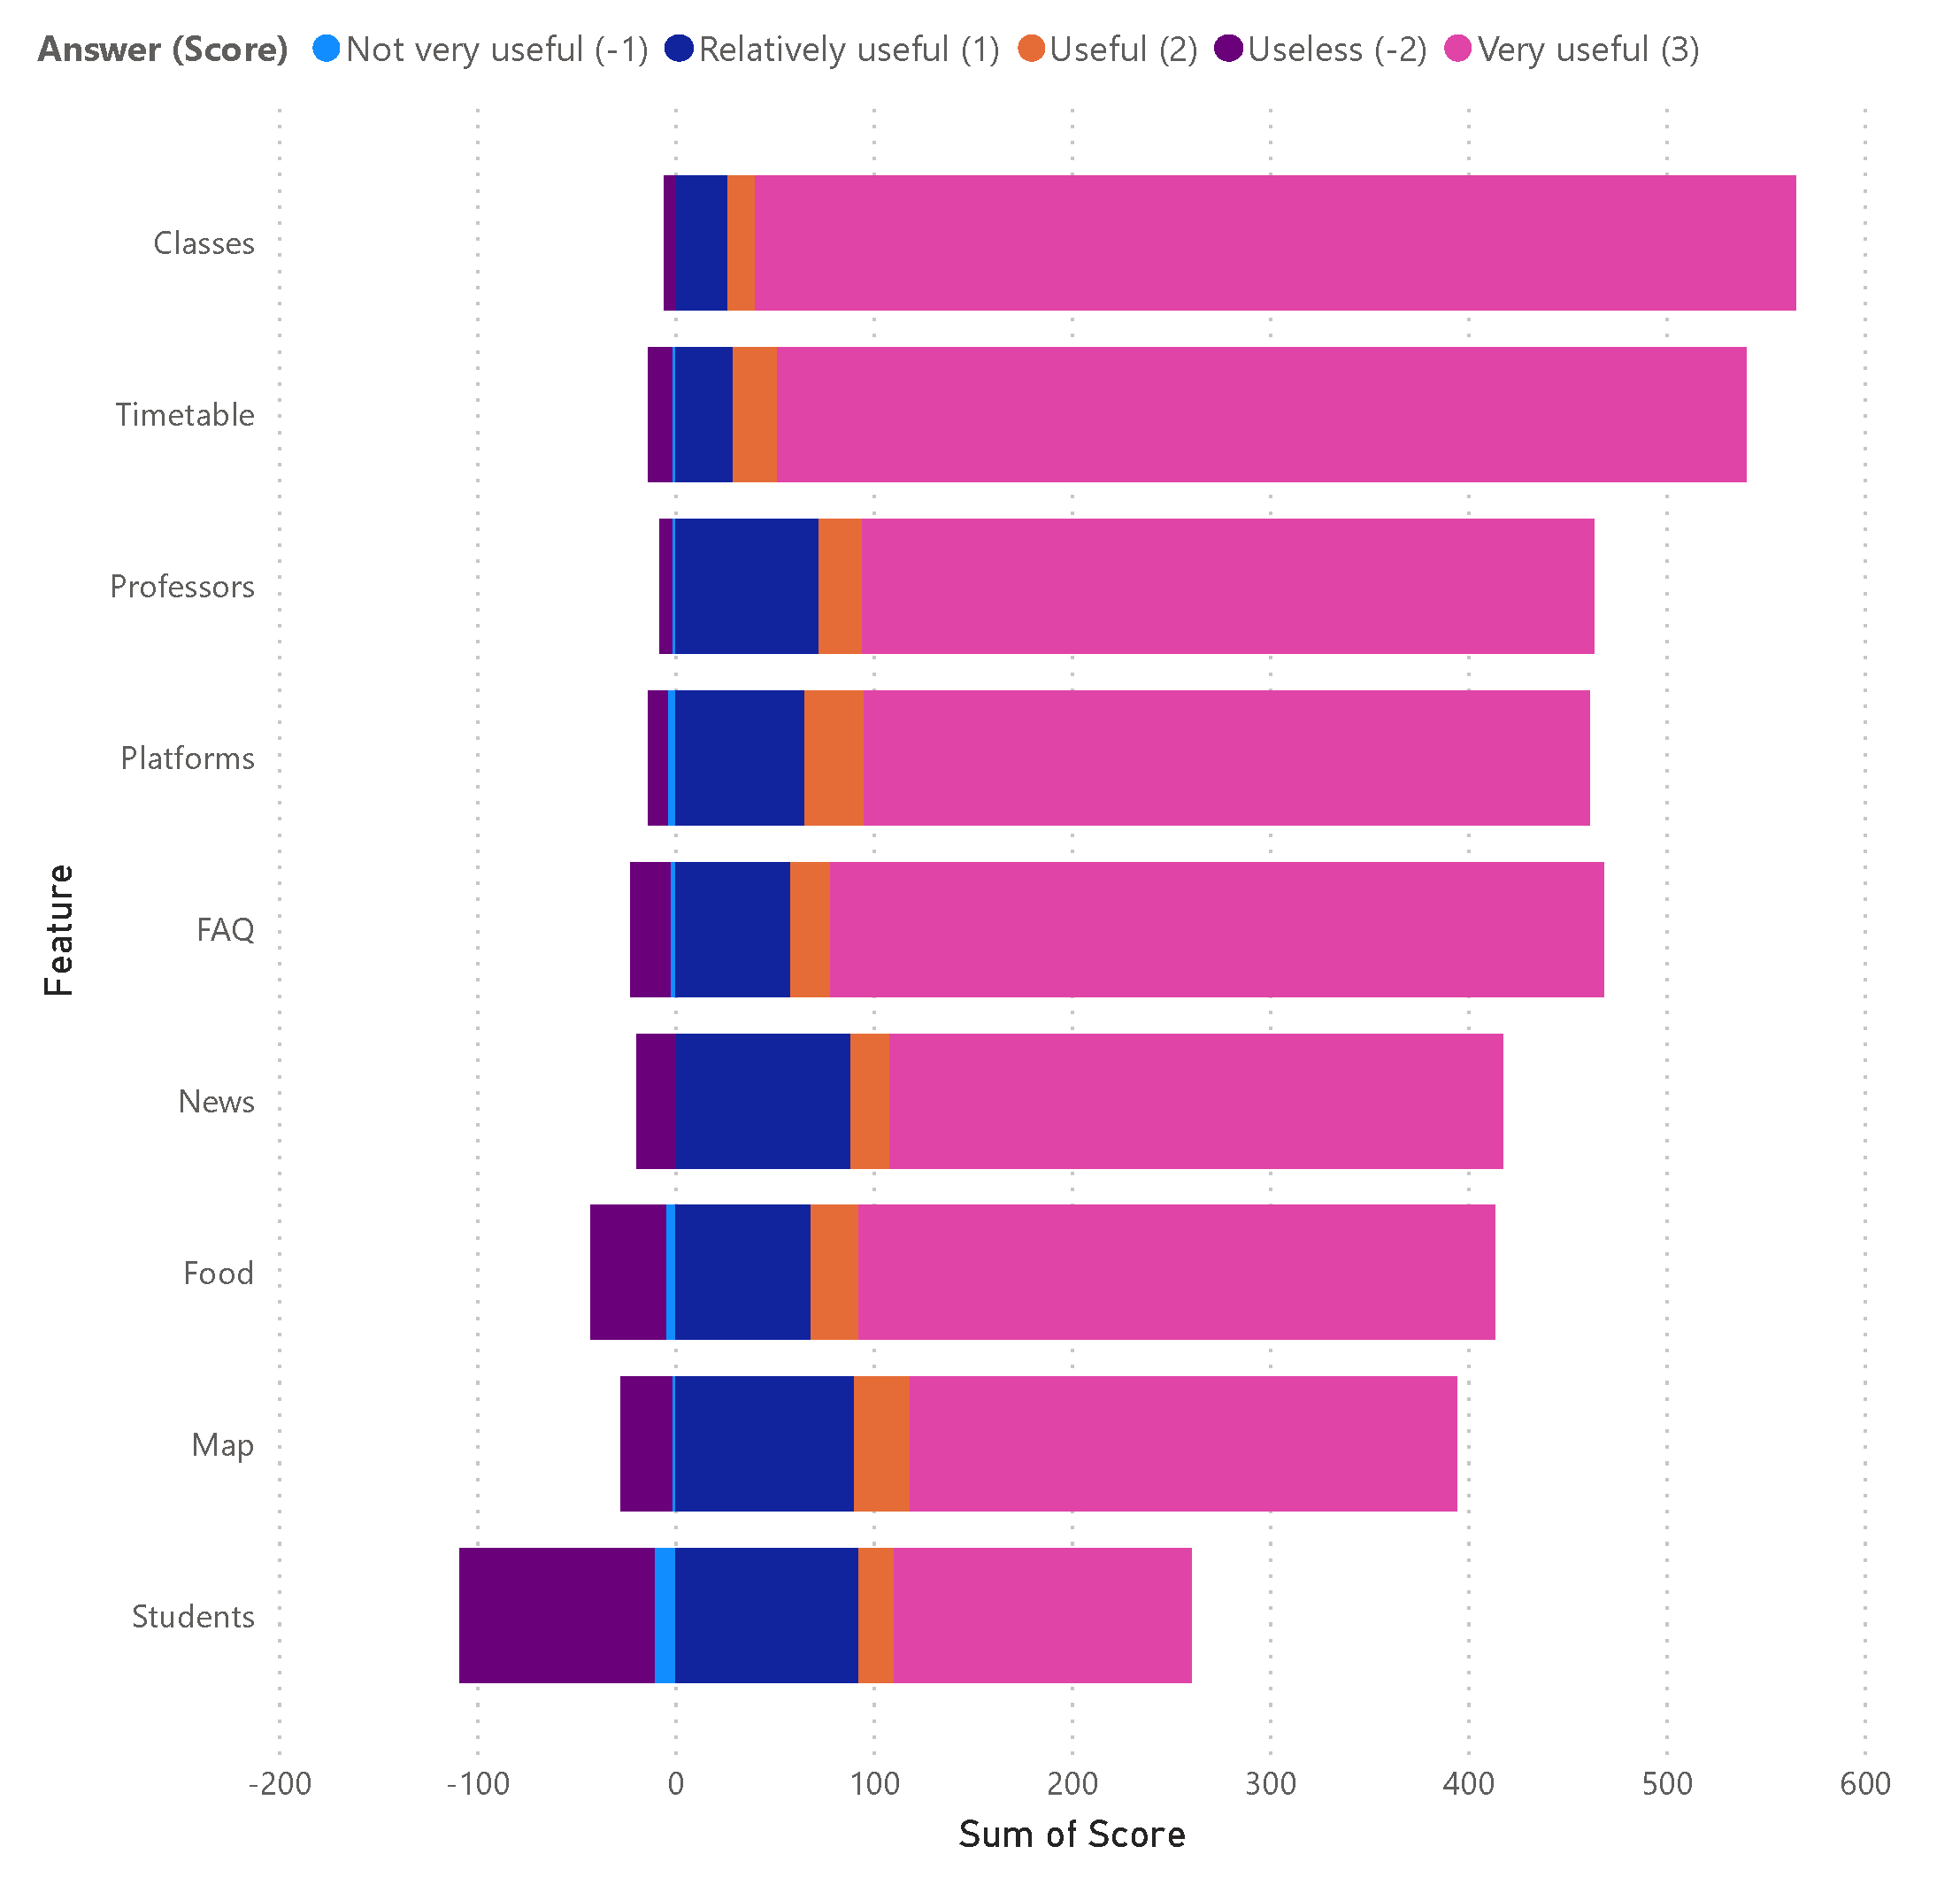
\includegraphics[height=0.5\textheight]{figures/charts/survey/features.pdf}
    \caption{Preferred app features for survey respondents}
    \label{3:fig:features}
\end{figure}

The vast majority of students considered information and resources for classes and a timetable to be the most useful features.

In an open-ended question, students suggested other features, such as an estimated waiting time for the canteens and a way to upload files for easy access. In terms of useful information that should be available in the app, some students suggested administrative information (about scholarships, or how to request specific documents) and feedback from other students about different classes and professors.

\subsection{Appearance} \label{3:appearance}

To find out how much we should prioritize coming up with an outstanding design for the application, we asked the students how important they believe the general appearance of an application to be. As seen in figure \ref{3:fig:appearance}, a vast majority of students believes appearance to be important or very important. Therefore, we need to focus as much as possible on the design step of the development process, described in chapter \ref{chapter4}.

\begin{figure}[ht]
    \centering
         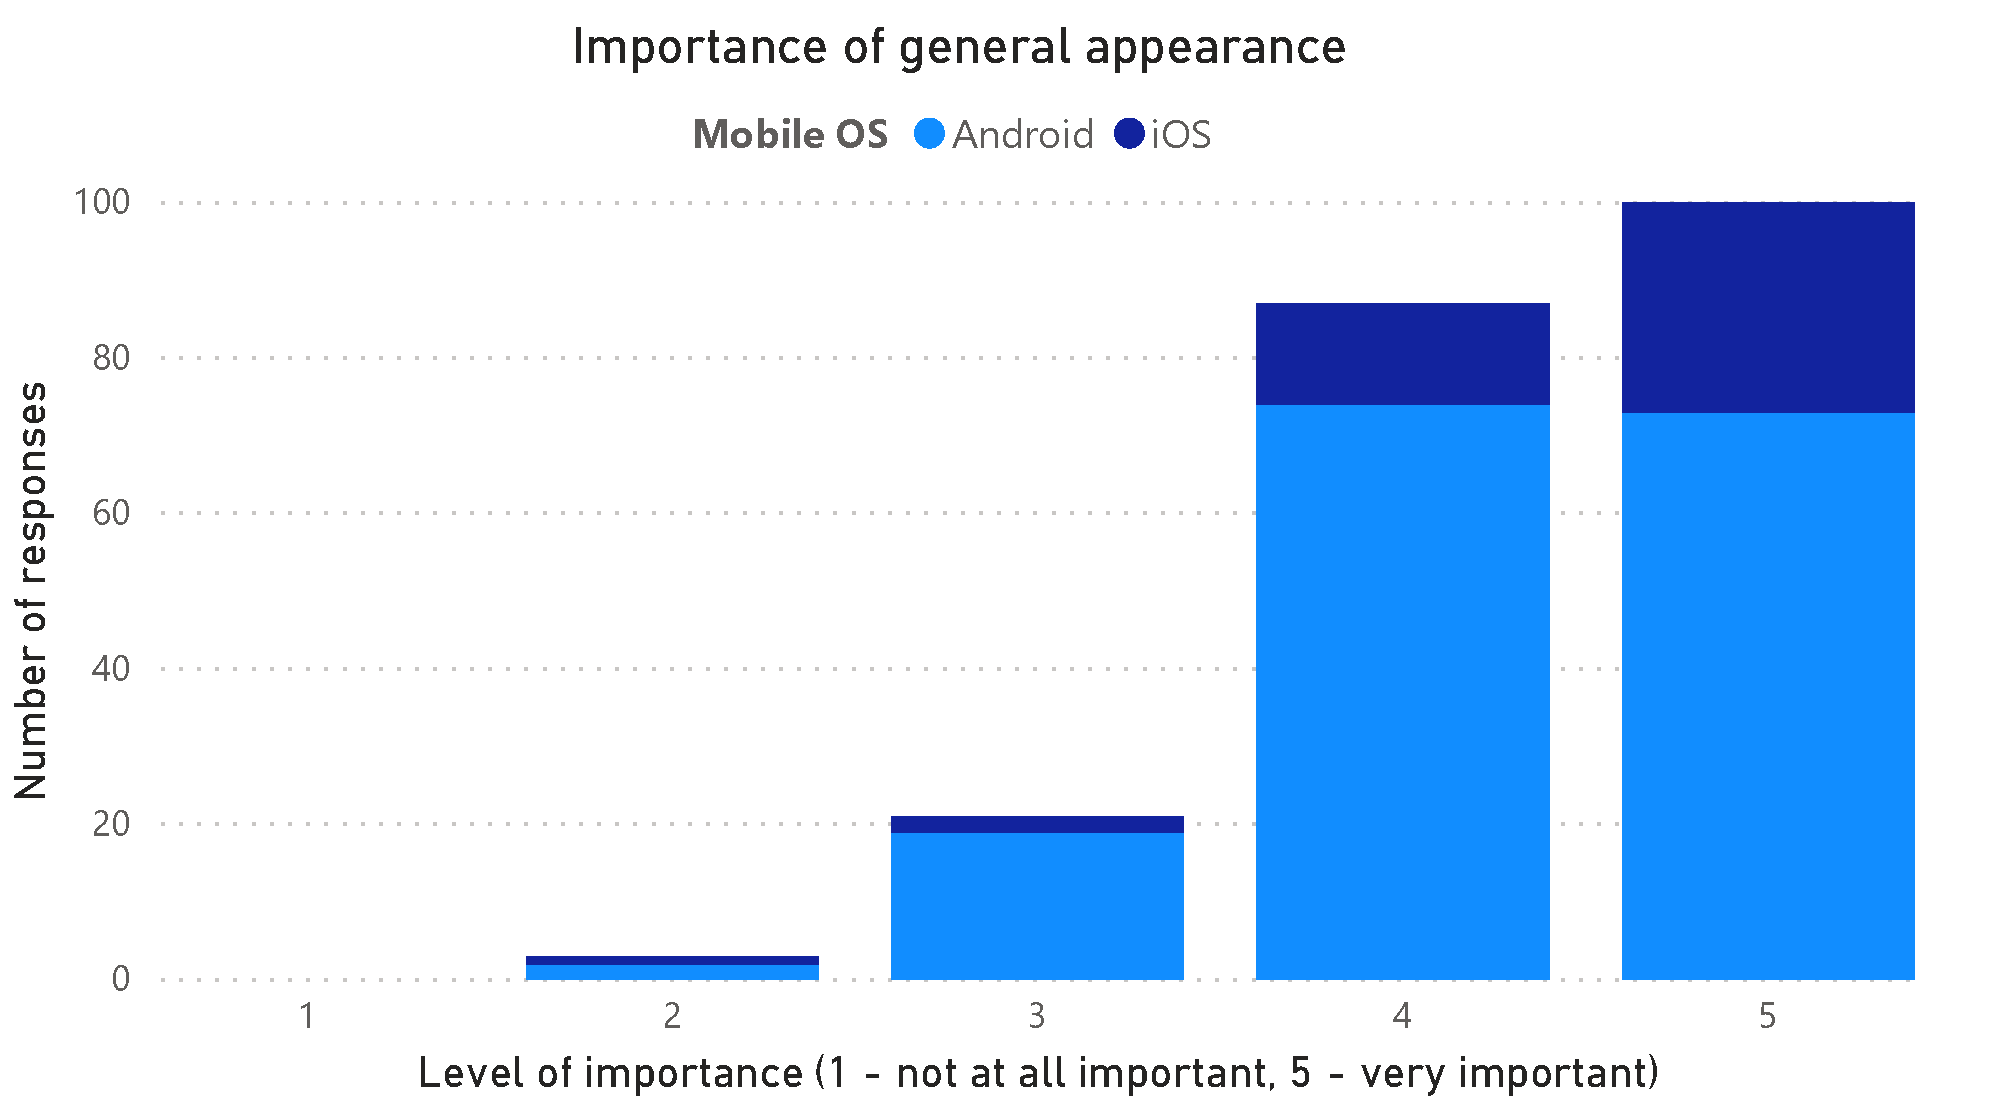
\includegraphics[width=0.95\textwidth]{figures/charts/survey/appearance.pdf}
    \caption{Importance of general appearance by \acrshort{os} for survey respondents}
    \label{3:fig:appearance}
\end{figure}

In an open-ended question, several students stressed that performance, as well as how smoothly an application works, are also essential factors. Additionally, some students mentioned that they prefer a simple, easy to understand menu that does not require a user to go through more than three steps to achieve a specific goal. Through this, they were referencing the 3-click rule of web design (as defined by Catherine E. Weeks\cite{weeks1997design}, "A person shouldn't have to click more than 3 times to find a piece of info"). However, we will not be focusing specifically on this arbitrary \acrshort{ux} requirement, because multiple studies\cite{porter2003testing}\cite{nielsen2006prioritizing} have proved it to be nothing other than a myth.

One difficulty in designing a cross-platform application is that different platforms have different design guidelines that tend to be quite different\cite{thirumala2017interaction}. To help decide on a common design language for the application, we asked students how important native appearance is for them in a mobile application. We split the answers based on the student's mobile \acrshort{os} of choice, as seen in figure \ref{3:fig:native_appearance}. A native look and feel to an application is more important for iOS users than for Android users. However, it does not seem to be as important as the overall appearance of an application. A visual comparison between native and non-native design can be seen in appendix \ref{a:native_cross}.

\begin{figure}[ht]
    \centering
         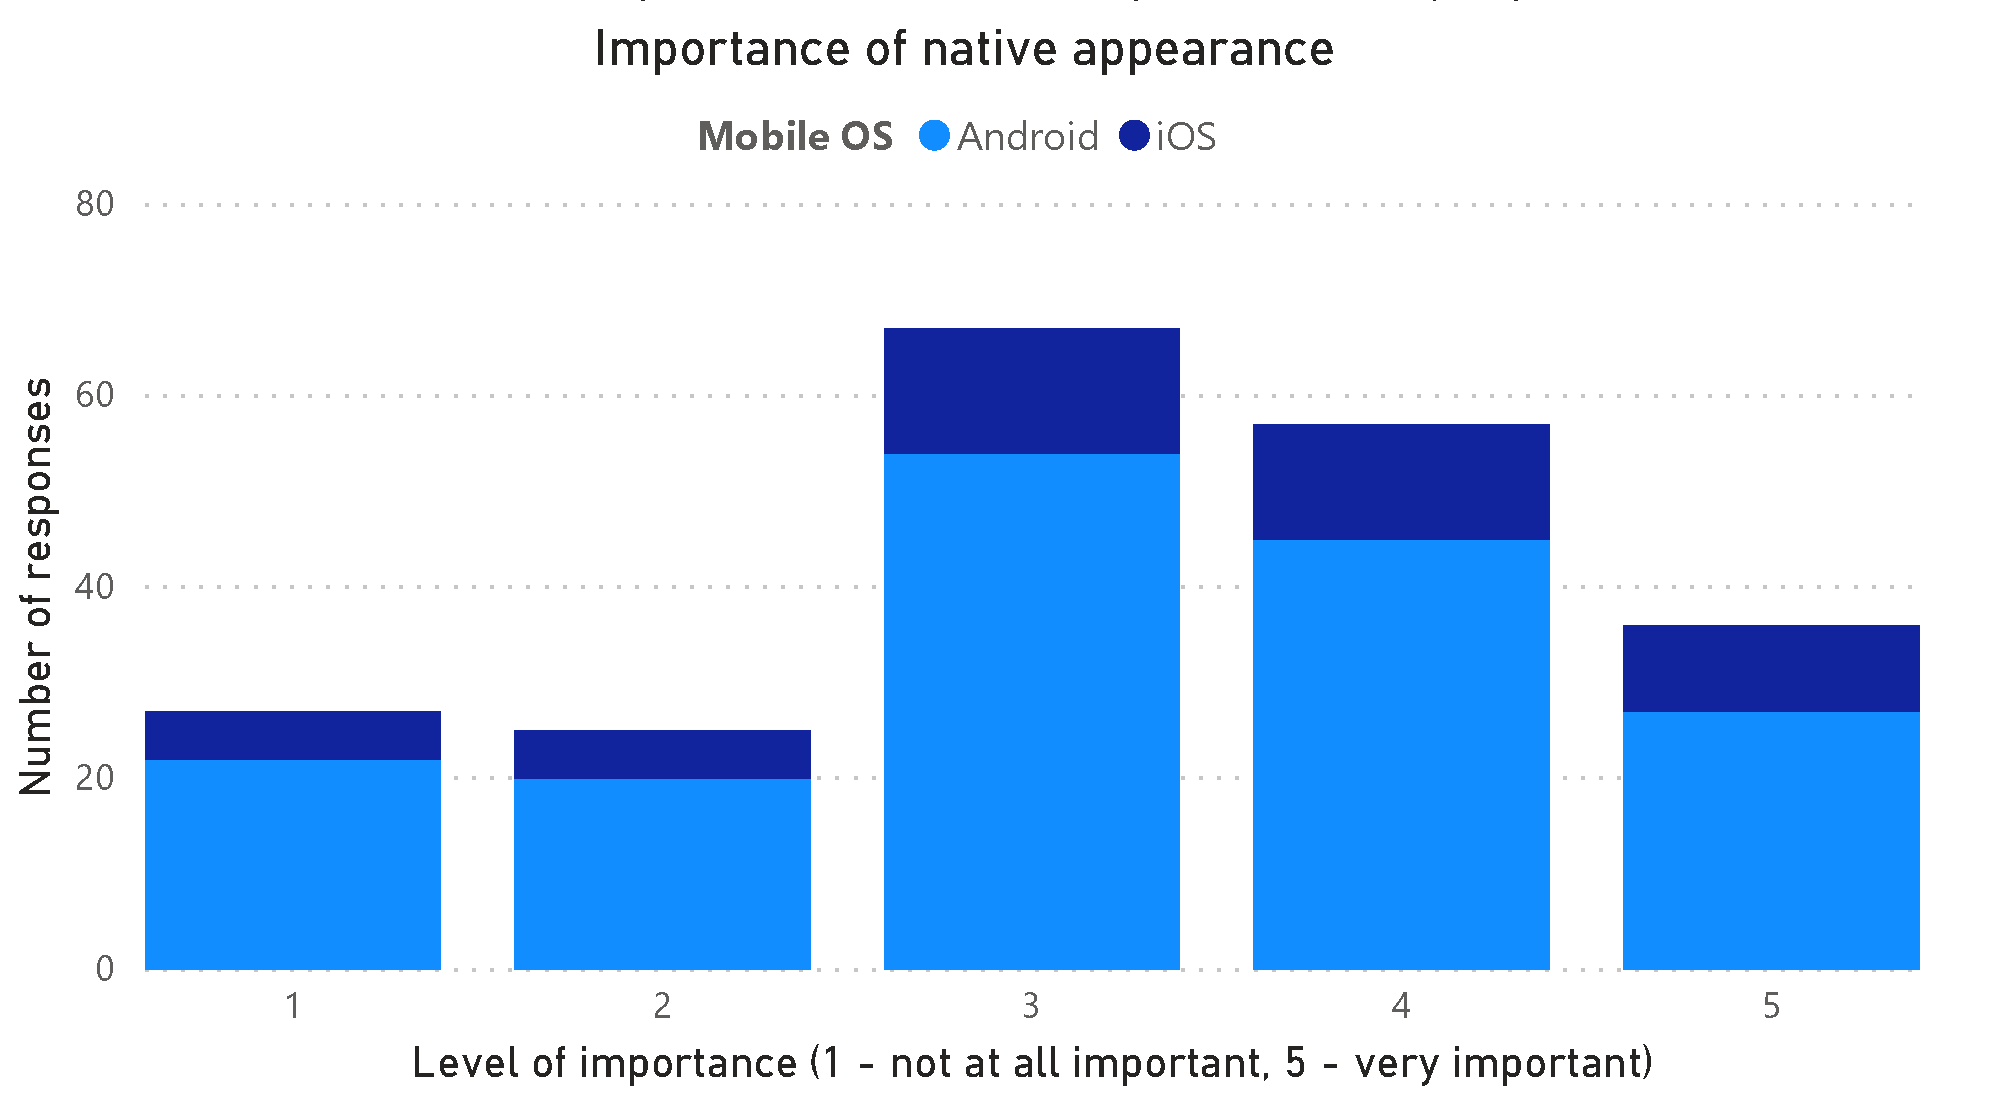
\includegraphics[width=0.95\textwidth]{figures/charts/survey/native_appearance.pdf}
    \caption{Importance of native appearance by \acrshort{os} for survey respondents}
    \label{3:fig:native_appearance}
\end{figure}

Based on these results, we will attempt to come up with a smooth, intuitive interface that is based on but does not strictly abide by the design rules of either iOS (Human Interface Guidelines\cite{apple2020human}) or Android platforms (Material Design\cite{google2020material}). We will make it our goal to find a proper middle-ground solution for our cross-platform application.

\subsection{Language} \label{3:language}

Finally, we asked students what language they prefer their mobile \acrshort{os} to be in, to find out whether we should prioritize localization for our application. Somewhat surprisingly for a faculty with almost exclusively native Romanian students, more than half of respondents said that they prefer their mobile language to be English, as shown in figure \ref{3:fig:language}. Only 2\% of respondents chose a different answer, with only one student mentioning German and the others saying that they do not prefer one language over the other.

\begin{figure}[ht]
    \centering
         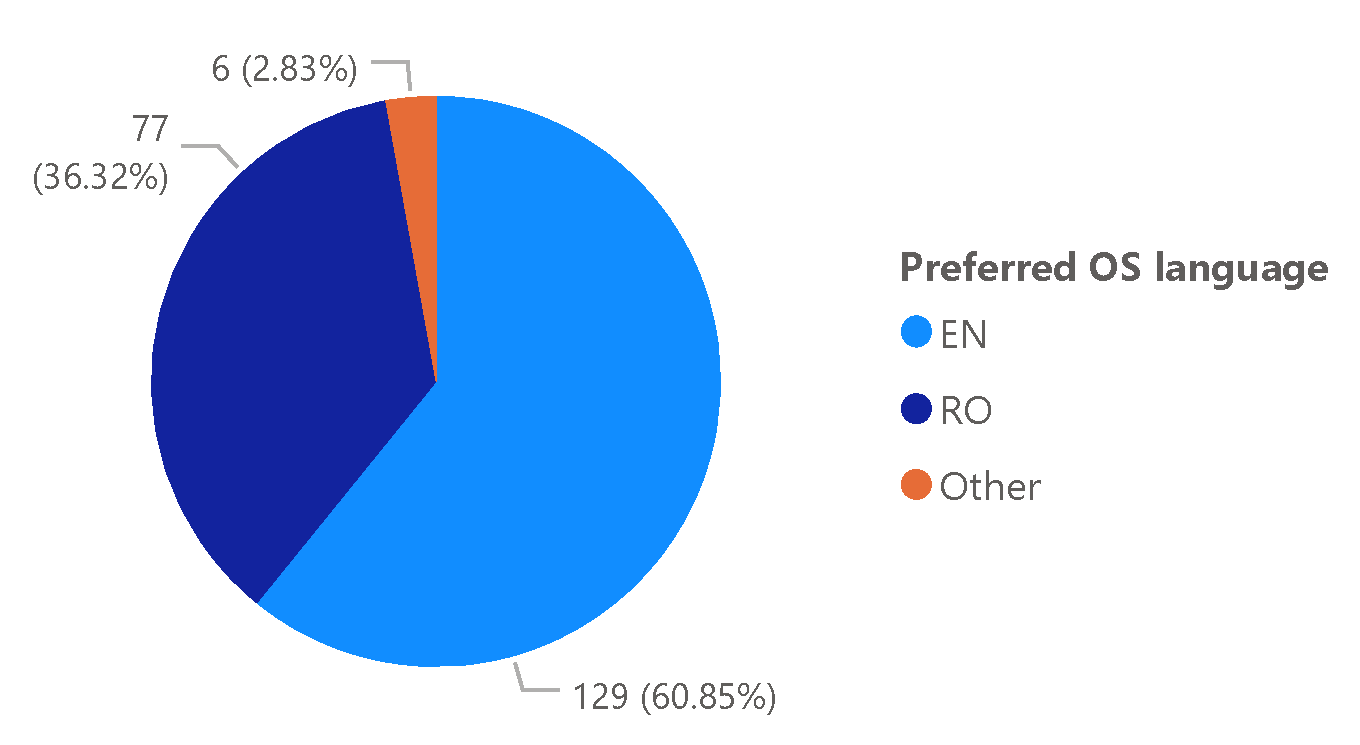
\includegraphics[height=0.2\textheight]{figures/charts/survey/language.pdf}
    \caption{Preferred \acrshort{os} language of survey respondents}
    \label{3:fig:language}
\end{figure}

With this data in mind, we know we need to pay close attention to our application's quality of localization. This feature is not just for the very few international students studying at \acrshort{acs}, but also for the many Romanian students who prefer their mobile devices and applications to be in English rather than their native language.